% настройки в preamble.inc
\documentclass[14pt]{extarticle}

\usepackage{indentfirst}

\usepackage[russian]{babel}
\usepackage[utf8]{inputenc}
\usepackage[T2A]{fontenc}

\usepackage{graphicx}  
\usepackage{amsfonts}
\usepackage{amsmath}
\usepackage{amssymb}
\usepackage{mathtools}
\usepackage{upgreek}
\usepackage{xfrac}
\usepackage{xcolor}



\usepackage{listings}

\lstset{
	captionpos=t,
	breaklines=true,         % автоматически переносить строки 
	breakatwhitespace=false, % переносить строки по пробелу
	%backgroundcolor=\color{mylightgray},rulecolor=\color{red},  % choose the background color; you must add \usepackage{color} or \usepackage{xcolor}; should come as last argument
	basicstyle=\footnotesize\ttfamily,        % the size of the fonts that are used for the code
	breakatwhitespace=false,         % sets if automatic breaks should only happen at whitespace
	breaklines=true,                 % sets automatic line breaking
	captionpos=t,                    % sets the caption-position to bottom
	commentstyle=\color{green},    % comment style
	extendedchars=false,              % lets you use non-ASCII characters; for 8-bits encodings only, does not work with UTF-8
	firstnumber=0,                % start line enumeration with line 1000
	frame=single,
	%rulesepcolor=\color{green},	                   % adds a frame around the code
	keepspaces=true,                 % keeps spaces in text, useful for keeping indentation of code (possibly needs columns=flexible)
	keywordstyle=\color{blue}\textbf,       % keyword style
	language=python,                 % the language of the code
	morekeywords={*,...},            % if you want to add more keywords to the set
	numbers=left,                    % where to put the line-numbers; possible values are (none, left, right)
	numbersep=5pt,                   % how far the line-numbers are from the code
	%numberstyle=\scriptsize\color{mygray}, % the style that is used for the line-numbers
	rulecolor=\color{black},         % if not set, the frame-color may be changed on line-breaks within not-black text (e.g. comments (green here))
	showspaces=false,                % show spaces everywhere adding particular underscores; it overrides 'showstringspaces'
	showstringspaces=false,          % underline spaces within strings only
	showtabs=false,                  % show tabs within strings adding particular underscores
	stepnumber=1,                    % the step between two line-numbers. If it's 1, each line will be numbered
	%stringstyle=\color{mymauve},     % string literal style
	tabsize=4,	                   % sets default tabsize to 2 spaces
	%title=\lstname                   % show the filename of files included with \lstinputlisting; also try caption instead of title
}

\lstset{
	captionpos=t,
	breaklines=true,         % автоматически переносить строки 
	breakatwhitespace=false, % переносить строки по пробелу
	%backgroundcolor=\color{mylightgray},rulecolor=\color{red},  % choose the background color; you must add \usepackage{color} or \usepackage{xcolor}; should come as last argument
	basicstyle=\footnotesize\ttfamily,        % the size of the fonts that are used for the code
	breakatwhitespace=false,         % sets if automatic breaks should only happen at whitespace
	breaklines=true,                 % sets automatic line breaking
	captionpos=t,                    % sets the caption-position to bottom
	commentstyle=\color{green},    % comment style
	extendedchars=false,              % lets you use non-ASCII characters; for 8-bits encodings only, does not work with UTF-8
	firstnumber=0,                % start line enumeration with line 1000
	frame=single,
	%rulesepcolor=\color{green},	                   % adds a frame around the code
	keepspaces=true,                 % keeps spaces in text, useful for keeping indentation of code (possibly needs columns=flexible)
	keywordstyle=\color{blue}\textbf,       % keyword style
	language=SQL,                 % the language of the code
	morekeywords={*,...},            % if you want to add more keywords to the set
	numbers=left,                    % where to put the line-numbers; possible values are (none, left, right)
	numbersep=5pt,                   % how far the line-numbers are from the code
	%numberstyle=\scriptsize\color{mygray}, % the style that is used for the line-numbers
	rulecolor=\color{black},         % if not set, the frame-color may be changed on line-breaks within not-black text (e.g. comments (green here))
	showspaces=false,                % show spaces everywhere adding particular underscores; it overrides 'showstringspaces'
	showstringspaces=false,          % underline spaces within strings only
	showtabs=false,                  % show tabs within strings adding particular underscores
	stepnumber=1,                    % the step between two line-numbers. If it's 1, each line will be numbered
	%stringstyle=\color{mymauve},     % string literal style
	tabsize=4,	                   % sets default tabsize to 2 spaces
	%title=\lstname                   % show the filename of files included with \lstinputlisting; also try caption instead of title
}


\usepackage{enumerate}
%\usepackage{multirow}
%\usepackage{tikz}
%\usetikzlibrary{arrows,positioning,shadows}
%\usepackage{paralist,array}

\usepackage{geometry}
\geometry{right=20mm}
\geometry{left=30mm}
\geometry{bottom=20mm}
\geometry{ignorefoot}% считать от нижней границы текста

\setlength{\parindent}{1.25 cm}
\setlength{\parskip}{1ex}
\renewcommand{\baselinestretch}{1.5}

\usepackage[toc,page]{appendix}

\usepackage{titlesec}
\titleformat{\section}
{\normalfont\fontsize{14}{14}\bfseries\centering}{\thesection}{1em}{}
\titleformat{\subsection}
  {\normalfont\fontsize{14}{14}\bfseries}{\thesubsection}{1em}{}

\makeatletter
\newcommand\subsubsubsection{\@startsection{paragraph}{4}{\z@}{-2.5ex\@plus -1ex \@minus -.25ex}{1.25ex \@plus .25ex}{\normalfont\normalsize\bfseries}}
\newcommand\subsubsubsubsection{\@startsection{subparagraph}{5}{\z@}{-2.5ex\@plus -1ex \@minus -.25ex}{1.25ex \@plus .25ex}{\normalfont\normalsize\bfseries}}
\makeatother


\usepackage[intoc]{nomencl}
\renewcommand{\nomname}{Обозначения и сокращения}
\makenomenclature

%Подписи
\usepackage		[margin		= 10	pt,
%					font		= footnotesize, 
					labelfont	= bf, 
					labelsep	= endash, 
					labelfont	= bf,
%					textfont	= sl,
					margin		= 0 	pt,  
					aboveskip 	= 4		pt, 
					belowskip 	= -6	pt,
					figurename= Рисунок] {caption}
\usepackage		[margin		= 10	pt,
					font		= footnotesize, 
					labelfont	= bf, 
					labelsep	= endash, 
					labelfont	= bf,
					textfont	= sl,
					margin		= 0 	pt,  
					aboveskip 	= 4		pt, 
					belowskip 	= 6	pt]	{subcaption}


\newcommand\Referat{%реферат
	\chapter*{Реферат}%
}

\addto\captionsrussian{%
	\def\contentsname{%
		Содержание}%
	\def\bibname{%
		Список~
		использованных~
		источников}%
}

\usepackage{enumitem}
\usepackage{indentfirst}
\usepackage{gensymb}
\usepackage{enumerate}
\usepackage{float}


\graphicspath{{images/}}
\begin{document}

\setcounter{page}{3}

% СОДЕРЖАНИЕ 
\clearpage
\tableofcontents

% ВВЕДЕНИЕ
\clearpage
\section*{Введение}
\addcontentsline{toc}{section}{Введение}
Задача по сбору и анализу трафика может возникнуть в различных ситуациях. Например, при наблюдении за поведением пользователей во внутренней сети, попытке отследить вредоносное программное обеспечение, обращающееся к внешнему сервису, или при контроле квоты использования интернета. Большой объем данных, проходящих через сетевые узлы, накладывает некоторые ограничения на инструменты, используемые при решении поставленной задачи.
	\\ \indent Целью данной работы является реализация программного комплекса для сбора, хранения и анализа информации о трафике, проходящего через некоторый сетевой узел.

Для достижения поставленной цели необходимо решить следующие задачи:
\begin{itemize}
	\item проанализировать предметную область;
	\item спроектировать программный комплекс;
	\item реализовать спроектированную систему.
\end{itemize}

% АНАЛИТИЧЕСКАЯ ЧАСТЬ
\clearpage
\section{Аналитический раздел}
В данном разделе будет поставлена задача, рассмотрены требования к системе и проведен анализ существующих решений.

\subsection{Постановка задачи}
Необходимо разработать программный комплекс, предоставляющий возможность собирать, хранить и просматривать информацию о трафике, проходящем через сетевой узел.

Предусмотреть наличие нескольких ролей пользователей с разным уровнем привилегий:
\begin{itemize}
	\item пользователь "Гость"\ с возможностью просмотра базовых таблиц;
	\item пользователь "Аналитик"\  с возможностью запуска сложных запросов и наличием тех же прав, что и у "Гость";
	\item пользователь "Администратор"\  с возможностью управления аккаунтами пользователей и наличием тех же прав, что и у "Аналитик".
\end{itemize}

\subsection{Требования к системе}
\begin{itemize}
	\item система должна обладать возможностью масштабирования на несколько сетевых узлов, кластеров хранения данных;
	\item необходимо обеспечить долгосрочное хранение больших объемов данных (трафик за несколько лет) с сохранением возможности поиска предыдущих записей
		за приемлемое время;
	\item предусмотреть возможность непрерывной работы подсистемы сбора данных в течении длительного времени.
\end{itemize}

\subsection{ Общие сведения }
Информация о трафике обычно представляется с помощью NetFlow протокола\cite{netflow}. Существуют различные версии протокола, но принцип работы у всех них один. Для сбора данных с помощью NetFlow используют следующие компоненты:
\begin{itemize}
	\item сенсор;
	\item коллектор;
	\item анализатор.
\end{itemize}
\indent \indent Сенсор служит для сбора статистики о проходящем через него трафике. Данные, собранные сенсором отправляются в коннектор, который агрегирует данные с нескольких сенсоров и записывает их в хранилище. Анализатор предоставляет возможность работы с данными. Схема архитектуры NetFlow представлена на рисунке \ref{netflow}.
\begin{figure}[H]
	\centering
	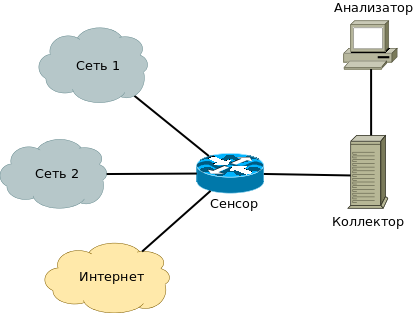
\includegraphics[scale=0.5]{netflow.png}
	\caption{Архитектура NetFlow.}
	\label{netflow}
\end{figure}

\subsection{ Анализ существующих решений}
Исходя из изложенных выше сведений можно выделить два направления поиска возможного решения:
\begin{itemize}
	\item приложение, реализующее в себе все компоненты архитектуры NetFlow;
	\item система, использующая отдельные компоненты вместе.
\end{itemize}

\subsubsection{ Приложение }
По первому направлению сравнения можно выделить два самых видных решения:
\begin{itemize}
	\item Wireshark;
	\item tcpdump.
\end{itemize}

\subsubsubsection{Wireshark}
Бесплатный, мультиплатформенный (работает на Windows, macOS и семействе Linux) анализатор трафика с открытым исходным кодом, предоставляющий возможность быстро проанализировать трафик сети\cite{wireshark}. Есть возможность фильтровать и сортировать трафик. Имеет интуитивно понятный и информативный интерфейс. Однако позволяет работать только с локальными интерфейсами, а записанные данные сохраняет в простой файл, что делает его неприменимым для долгосрочного сбора данных и не дает возможности масштабирования.
\subsubsubsection{tcpdump}
Бесплатный анализатор трафика\cite{tcpdump}. Работает на Linux, но есть несколько портов для Windows. Предоставляет базовую функциональность через консольный интерфейс. Минусы такие же как и у Wireshark - отсутствие возможности масштабирования и работа только с локальными интерфейсами.

В таблице \ref{CompareWP} представлено сравнение Wireshark и tcpdump
\begin{table}[H]
\caption{Cравнение Wireshark и tcpdump.}
\begin{center}
\begin{tabular}{ |p{5cm} |p{5cm}| p{5cm} |}
\hline
 & Wireshark & tcpdump  \\ \hline 
Возможность просмотра информации о трафике & + & + \\ \hline 
Наличие графического интерфейса & + & -  \\ \hline 
Возможность записи данных в бд & - & - \\ \hline 
Возможность отправки данных & - & - \\ \hline 
Работа с удаленными интерфейсами & - & - \\ \hline 
Разграничение сбора и анализа информации & - & - \\ \hline
\end{tabular}
\end{center}
\label{CompareWP}
\end{table}

Как видно, готовые программы анализа информации о трафике имеют общие недостатки, не позволяющие использовать их для решения поставленной задачи.
\subsubsection{ Система }
По второму направлению сравнения выделить готовых систем не удалось, но можно выделить некоторые популярные решения отдельных модулей.

\subsection{Анализ моделей СУБД}
Модель данных определяет логическую структуру базы данных, то, каким образом данные могут храниться, организовываться и обрабатываться. Существуют два больших класса СУБД - SQL и NoSQL.

\subsubsection{SQL}
Наиболее популярным и самым распространенным типом СУБД является РСУБД (реляционная СУБД) или SQL-СУБД. Такие СУБД построены на основе реляционной модели, поддерживают стандарт SQL и поэтому имеют много схожих характеристик. \\
\indent В реляционной модели данные представляются в виде строк в таблицах, соотносящих атрибуты и значения. Реляционная модель строго определяет структуру данных, ограничения целостности над данными, теоретико-множественные операции над ними. В реалиционной модели определены два базовых требования обеспечения целостности:
\begin{itemize}
 \item ссылочная целостность (гарантия отсутствия ссылок на несуществующие объекты);
 \item целостность сущностей (гарантия уникальности объектов).
\end{itemize}
\indent \indent Вследствие вышесказанного SQL СУБД хорошо проходит для хранения данных, имеющих строго определенную структуру.

\subsubsection{NoSQL}
NoSQL СУБД появились не так давно, но уже обрели достаточно большую популярность в силу своих особенностей. NoSQL СУБД не имеют одной общей модели данных, единственное, что их объединяет это базированность не на основе реляционной модели. \\
\indent У NoSQL СУБД есть ряд преимуществ над SQL СУБД:
\begin{itemize}
 \item возможность хранения больших объемов неструктурированной информации;
 \item большая скорость обработки больших объемов данных;
 \item отсутствие проблем с масштабируемостью.
\end{itemize}

\indent \indent NoSQL СУБД хорошо подходят для хранения больших данных, так как имеют большую скорость обработки, позоляют легко смасштабировать систему и позволяют хранить неструктурированную информацию.


В таблице \label{CompareSQL} Представлено сравнение SQL и NoSQL СУБД. 
\begin{table}[H]
\caption{Cравнение SQL и NoSQL.}
\begin{center}
\begin{tabular}{ |p{5cm} |p{5cm}| p{5cm} |}
\hline
 & SQL & NoSQL  \\ \hline 
Поддержка SQL & + & частично \\ \hline 
Легкость масштабирования & - & +  \\ \hline 
Высокая скорость обработки больших данных & - & + \\ \hline 
Поддержка связанности & + & - \\ \hline 
Поддержка хранимых процедур и тригеров & + & - \\ \hline 
\end{tabular}
\end{center}
\label{CompareSQL}
\end{table}

\indent Исходя из требований к системе и сущности обрабатываемых данных был выбран NoSQL подход.

\subsection{Вывод}
В данном разделе была поставлена задача, рассмотрены требования к системе, проанализированы существующие решения.


%КОНСТРУКТОРСКИЙ РАЗДЕЛ
\clearpage
\section{Конструкторский раздел}
В данном разделе будут спроектированы база данных и приложение.


\subsection{Сценарии использования}
Необходимо формализовать требуемую функциональность. 
\subsubsection{Гость}
У пользователя с ролью "Гость"\ есть только самые базовые права - права на просмотр существующие данные, без возможности их как-либо менять или делать сложные запросы.
Разрешаемые действия:
\begin{itemize}
	\item[1)] просмотр всех источников;
	\item[2)] просмотр всех типов источников;
	\item[3)] просмотр всех владельцев источников;
	\item[4)] просмотр всех точек назначения;
	\item[5)] просмотр всех типов точек назначений;
	\item[6)] просмотр потока данных за последние n минут.
\end{itemize}

\subsubsection{Аналитик}
Функциональность, предоставляемая аналитику расширяет возможности гостя:
\begin{itemize}
	\item[1)] просмотр потока определенного типа;
	\item[2)] просмотр потока из определенного интервала;
	\item[3)] получение суммы трафика от источников.
\end{itemize}
\subsubsection{Администратор}
Администратор, помимо предоставляемого аналитику функционала, может управлять аккаунтами пользователей:
\begin{itemize}
	\item[1)] просмотреть всех пользователей;
	\item[2)] удалить пользователя;
	\item[3)] создать пользователя;
	\item[4)] выдать права пользователю;
	\item[5)] забрать права у пользователя.
\end{itemize}
\indent На рисунке \ref{usecase} приведена use-case диаграмма.
\begin{figure}[H]
	\centering
	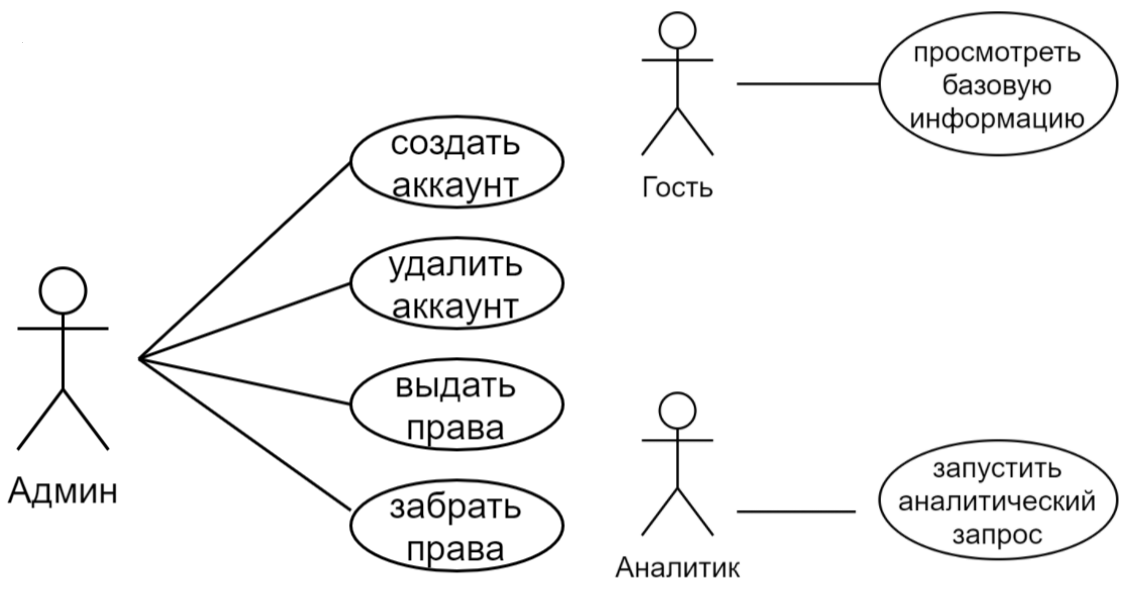
\includegraphics[scale=0.55]{usecase.png}
	\caption{Схема потоков данных системы.}
	\label{usecase}
\end{figure}

\subsection{Проектирование системы}
На этапе анализа были выделены три сущности:
\begin{itemize}
\item Сенсор
\item Коллектор
\item Анализатор
\end{itemize}

В проектируемой системе было решено использовать базу данных и клиентское приложение. На рисунке \ref{fullSCH} представлена схема потоков данных системы.

\begin{figure}[H]
	\centering
	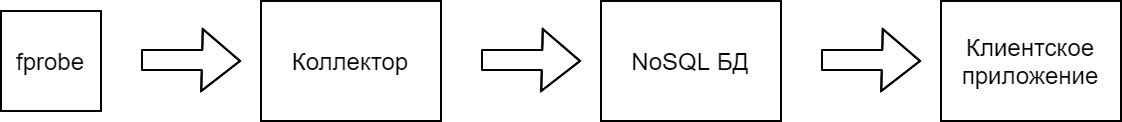
\includegraphics[scale=0.55]{conc.png}
	\caption{Схема потоков данных системы.}
	\label{fullSCH}
\end{figure}


\subsection{Проектирование базы данных}

Для проектирования базы данных необходимо выделить и описать сущности системы.
\subsubsection{Ролевая модель}
На уровне базы данных введены следующие роли:
\begin{itemize}
	\item[1)] guest;
	\item[2)] analyst;
	\item[3)] admin.
\end{itemize}
\indent \indent Права приведенных ролей совпадают с возможностями пользователей этой роли.

\subsubsection{Формализация сущностей системы}
На рисунке \ref{ER} представлена ER-диаграмма системы.
\begin{figure}[H]
	\centering
	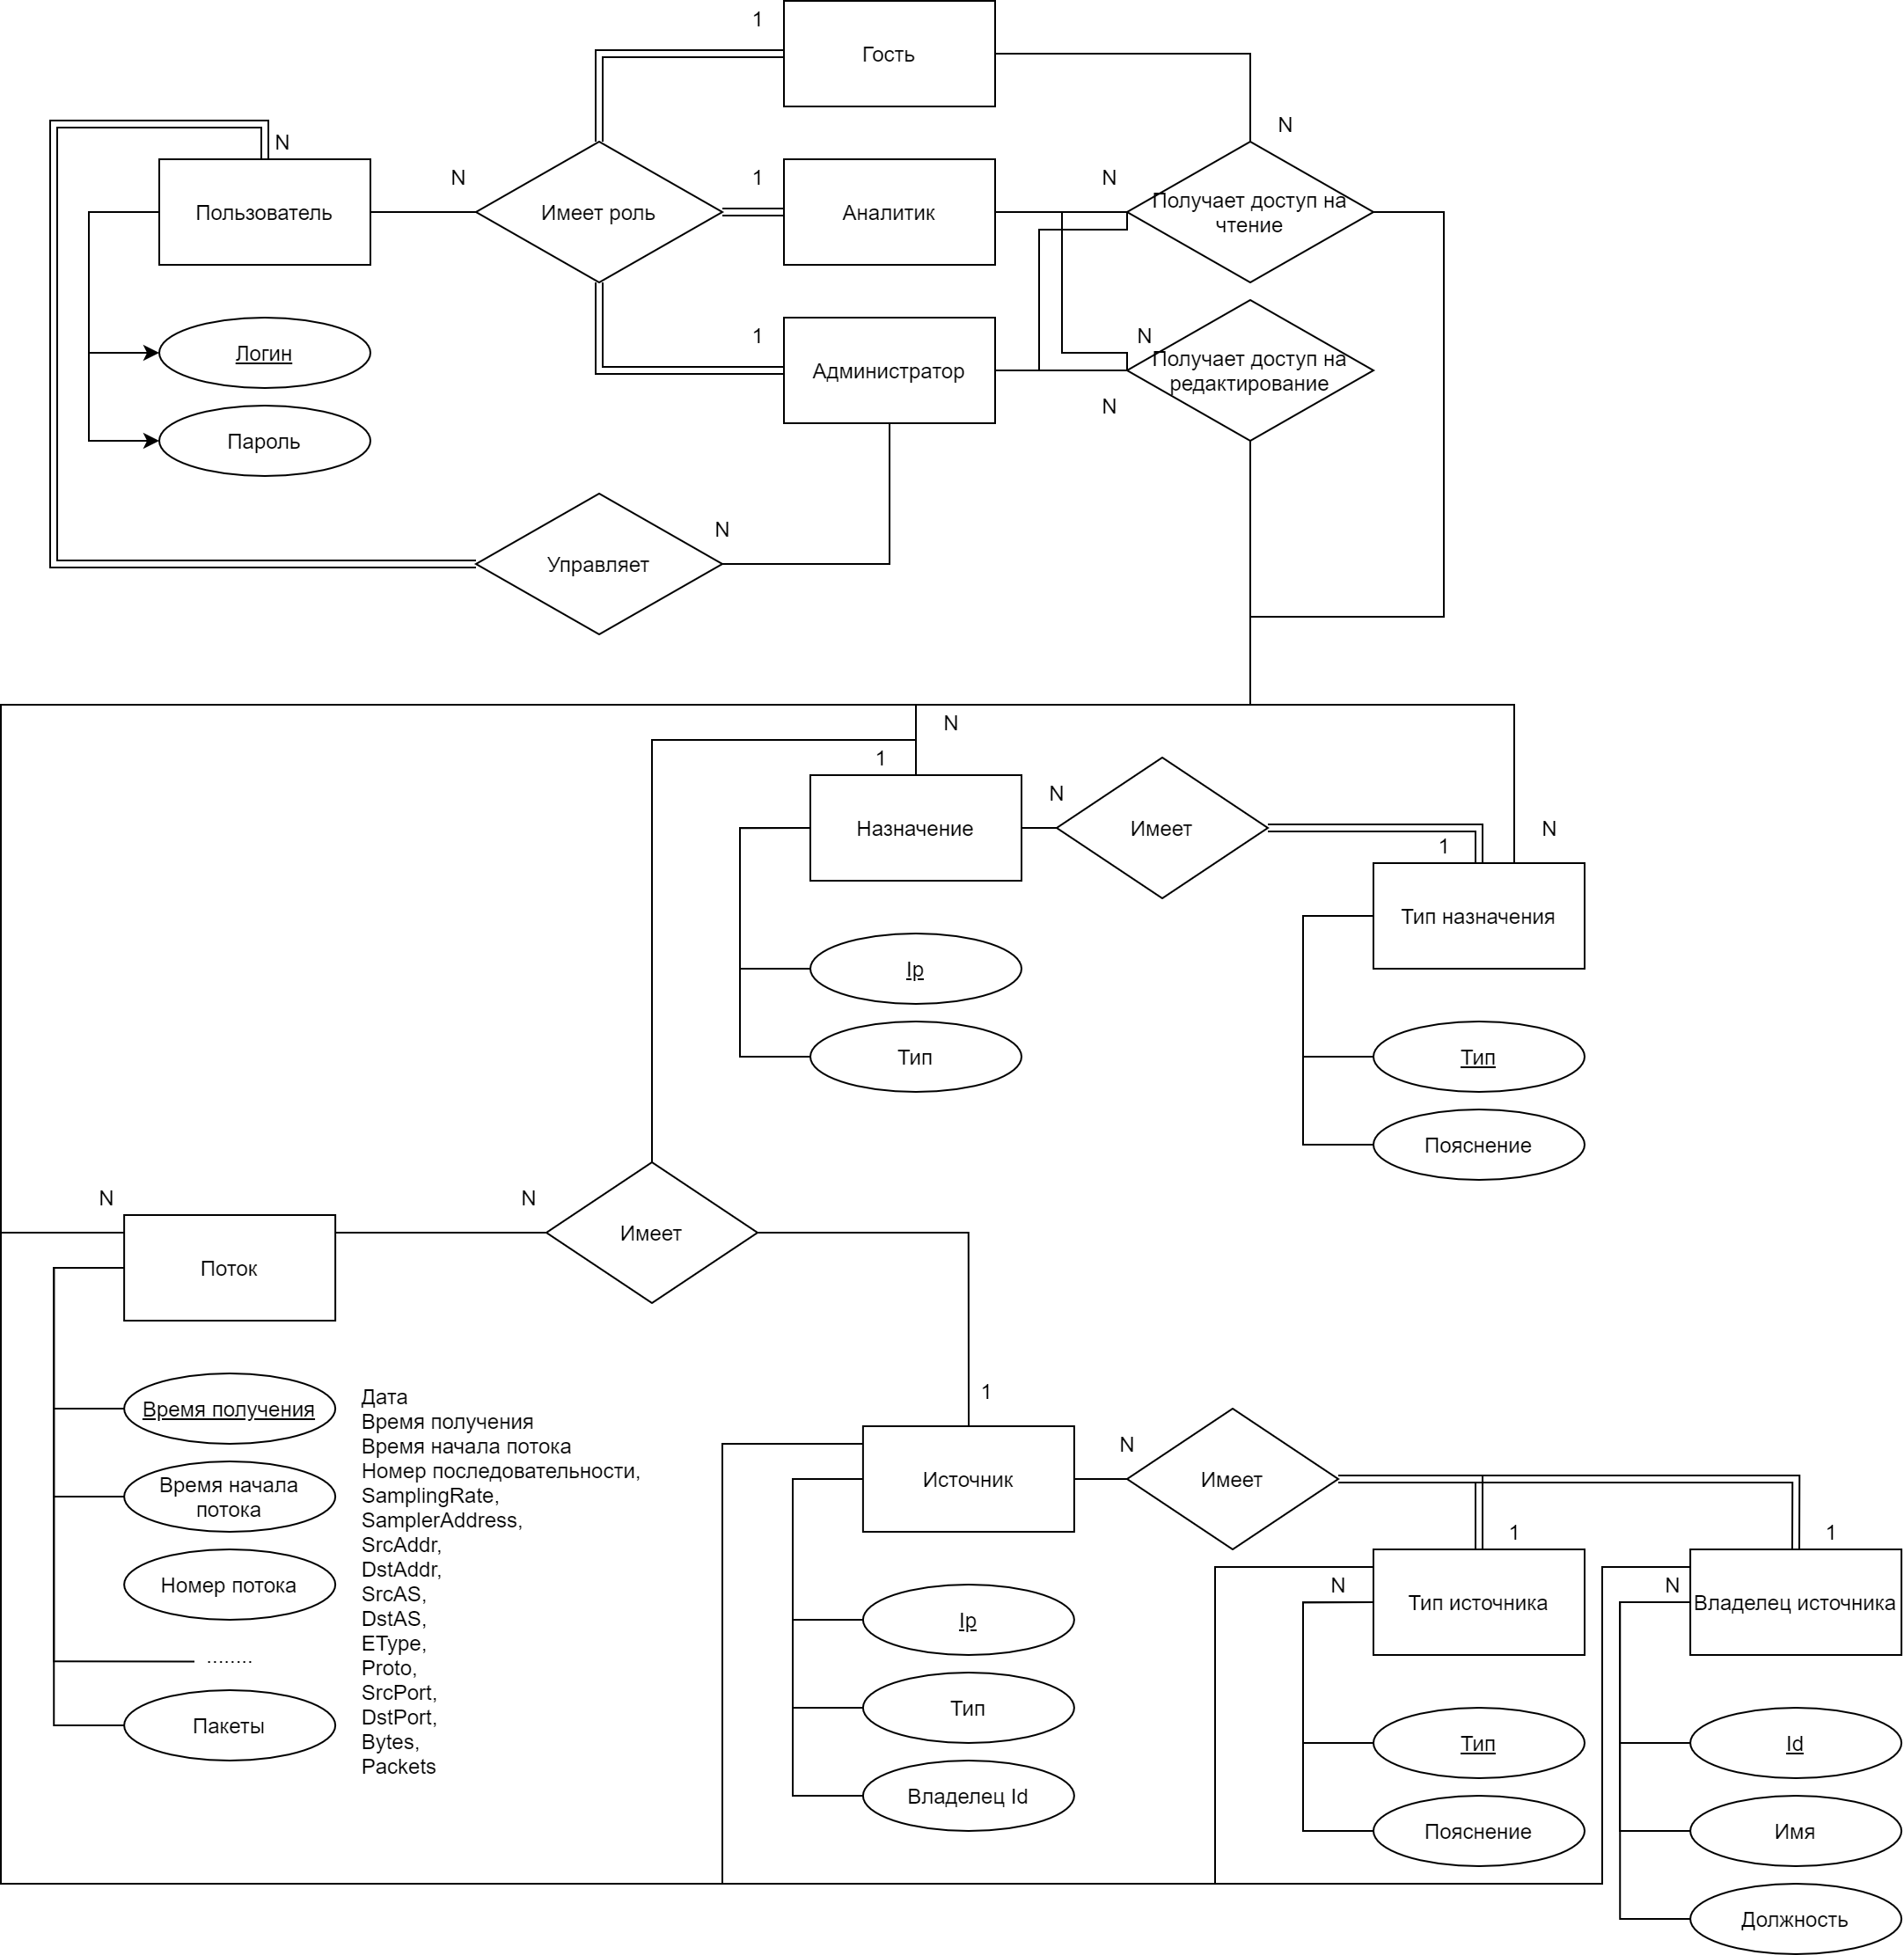
\includegraphics[scale=0.18]{ER.png}
	\caption{ER-диаграмма системы.}
	\label{ER}
\end{figure}
Выделенные сущности:
\begin{itemize}
	\item[1)] Пользователь - пользователь системы;
	\item[2)] Администратор, Гость, Аналитик - роли;
	\item[3)] Поток - поток данных;
	\item[4)] Источник - источник потока;
	\item[5)] Тип источника - тип источника;
	\item[6)] Владелец источника - так как предполагается, что мы находимся во внутренней сети, у источника есть известное нам расположение и владелец;
	\item[7)] Назначение - место назначение потока данных.
	\item[8)] Тип назначения - тип точки назначения.
\end{itemize}

\subsubsection{Материализованное представление}
Для того, чтобы автоматически сортировать потоки трафика, необходимо создать материализованное представление, способное агрегировать информацию из нескольких таблиц для записи в таблицу агрегированных данных.

\subsection{Проектирование приложения}
Приложение анализатор NetFlow спроектировано по архитектурному паттерну MVC.
Были выделены три компонента:
\begin{enumerate}
	\item доступа к данным;
	\item бизнес-логики;
	\item интерфейса.
\end{enumerate}
\indent \indent Компонент доступа к данным предоставляет интерфейс для взаимодействия с базой данных. В компоненте бизнес-логики содержатся контроллеры, использующиеся в компоненте интерфейса.
\subsection{Вывод}
В данном разделе были рассмотрены сценарии использования, спроектирована система и компоненты системы.

\newpage
%ТЕХНОЛОГИЧЕСКИЙ РАЗДЕЛ
\section{Технологический раздел}

В данном разделе будут выбраны средства реализации поставленной задачи, создана база данных и ролевая модель, разработаны компоненты и описан порядок работы.

\subsection{Выбор средств реализации поставленной задачи}
\subsubsection{Выбор сенсора}
Были выделены две утилиты, предоставляющие возможность сбора и отправки пакетов netflow: fprobe и nProbe. В таблице \ref{CompareProbe} представлено их сравнение

\begin{table}[H]
\caption{Сравнение netflow и nProbe.}
\begin{center}
\begin{tabular}{ |p{5cm} |p{5cm}| p{5cm} |}
\hline 
 & nProbe & fprobe  \\ \hline 
Бесплатный & - & + \\ \hline 

Возможность работать с различными версиями NetFlow  & v5/v9/IPFIX & v1/v5/v7  \\ \hline 
Мультиплатформен- ность & Linux, FreeBSD и Windows & Linux \\ \hline 
Поддержка IPv4/v6 & + & - \\ \hline
\end{tabular}
\end{center}
\label{CompareProbe}
\end{table}



\indent Так как утилита fprobe бесплатна и предоставляет всю необходимую функциональность для разработки была выбрана она.
 \subsubsection{Выбор СУБД}
Так как в аналитической части была выбрана модель данных NoSQL будут рассмотрены только NoSQL СУБД. \\
	Одной из известных NoSQL базой данных является Elasticksearch. Это документо-ориентированная база данных, разрабатываемая компанией Elastic и имеющая все плюсы NoSQL базы данных. Является частью так называемого ElastickStack - программного комплекса для записи, хранения и просмотра данных. В ElastickStack или ELK(Elasticksearch, Logstash, Kibana) - Logstash позволяет не терять данные в случае временного выхода из строя Elasticksearch, а Kibana визуализирует их. У Elasticksearch есть open-source версия с урезанной функциональностью под лицензией Apache 2.0, бесплатная версия под версий под лицензией Elastic и несколько коммерческих версий под лицензией Elastic License. \\
\indent	Другая NoSQL база данных Clickhouse является  \\ столбцово-ориентированной и её производительность выше чем у Elasticksearch\cite{clickhouse-elastic}. Разрабатывается компанией Yandex, является open-source под лицензией Apache 2.0\\
\indent В таблице \ref{CompareELCL} представлено их сравнение.

\begin{table}[H]
\caption{Cравнение Elasticksearch и ClickHouse.}
\begin{center}
\begin{tabular}{ |p{5cm} |p{5cm}|p{5cm} |}
\hline 
 & Elasticksearch & ClickHouse  \\ \hline 
NoSQL & + & + \\ \hline 
Парадигма & Документо-ориентированная & Столбцово-ориентированная \\ \hline 
Бесплатная & -/+ & +  \\ \hline 
Open-source & -/+ & + \\ \hline 
Скорость обработки больших данных & Большая & Ещё больше \\ \hline
\end{tabular}
\end{center}
\label{CompareELCL}
\end{table}

\indent Ввиду урезанной в open-source версии Elasticsearch функциональности (например, отсутствие ролевой модели), большей скорости работы с данными в ClickHouse, и специфики данных (в системе используются структурированные данные) был выбран Clickhouse.
\subsubsection{Выбор брокера}
Для агрегации данных с сенсоров нужна прослойка между базой данных и сенсорами, агрегирующая данные. В качестве такой прослойки было выбрано использовать брокер сообщений.\\
\indent Можно выделить два брокер сообщений для анализа. RedisMS и Kafka. \\
\indent Kafka -  распределенный горизонтально масштабируемый отказоустойчивый программный брокер сообщений. Приложения (генераторы) посылают сообщения (записи) на узел Kafka (брокер), и указанные сообщения обрабатываются другими приложениями, так называемыми потребителями. Указанные сообщения сохраняются, a потребители подписываются для получения новых сообщений. Kafka гарантирует, что все сообщения будут упорядочены именно в той последовательности, в которой поступили. Kafka не отслеживает, какие записи считываются потребителем и после этого удаляются, а просто хранит их в течение заданного периода времени. Потребители сами опрашивают Kafka, не появилось ли у него новых сообщений, и указывают, какие записи им нужно прочесть\cite{kafka-redis}. Между ClickHouse и Kafka существует нативная интеграция.\\
\indent
Приложения (publishers) посылают сообщения на узел RabbitMQ (exchange), при этом RabbitMQ отсылает обратно приложениям подтверждение, что сообщение получено. Получатели (consumers) постоянно соединены с RabbitMQ по TCP и ждут, когда RabbitMQ протолкнет (push) им сообщения. Получатели подтверждают получение сообщения или сообщают о неудаче. Если доставка неудачна, то RabbitMQ проталкивает сообщение до тех пор, пока оно не будет доставлено. После успешной доставки сообщение удаляется из очереди\cite{kafka-redis}. \\
\indent В таблице \ref{CompareREDKAF} представлено их сравнение.

\begin{table}[H]
\caption{Cравнение RabbitMQ и Kafka.}
\begin{center}
\begin{tabular}{ |p{5cm} |p{5cm}|p{5cm} |}
\hline 
 & Redis & Kafka\\ \hline 
Масштабируем & + & + \\ \hline 
Отказоустойчив & + & + \\ \hline 
Поддерживает UDP протокол получения пакетов & - & -  \\ \hline 
Существует коллектор для записи Netflow & - & +  \\ \hline 
Поддерживает интеграцию с ClickHouse & - & + \\ \hline 
\end{tabular}
\end{center}
\label{CompareREDKAF}
\end{table}


\indent Так как Kafka поддерживает интеграцию в ClickHouse без сторонних модулей и существует модуль для записи Netflow в Kafka (Goflow)\cite{Goflow}, был выбран брокер сообщений Kafka.

\subsubsection{Выбор инструментов для реализации приложения}

В качестве языка программирования был выбран язык C\#, так как он поддерживает парадигму ООП, имеет большой набор библиотек, легкий в использовании конструктор интерфейса для WinForms\cite{sharp}. \\
\indent В качестве среды разработки была выбрана "Microsoft Visual Studio 2019"\cite{vs}, поскольку она имеет много полезных возможностей при написании кода на C\#\cite{vs}. 

\subsubsection{Остальные выбранные технологии и инструменты}
\indent В качестве инструмента развертывания был выбран Docker, так как он позволяет быстро и без установки сторонних модулей развернуть приложение на новой машине. \\
\indent Разработка ведется на Linux Manjaro 5.11 И Windows 10.

\subsubsection{Диаграмма потока данных}
Для общего представления о системе на рисунке \ref{DataFlowEnd} представлена диаграмма потока данных с учетом используемых технологий.
\begin{figure}[H]
	\centering
	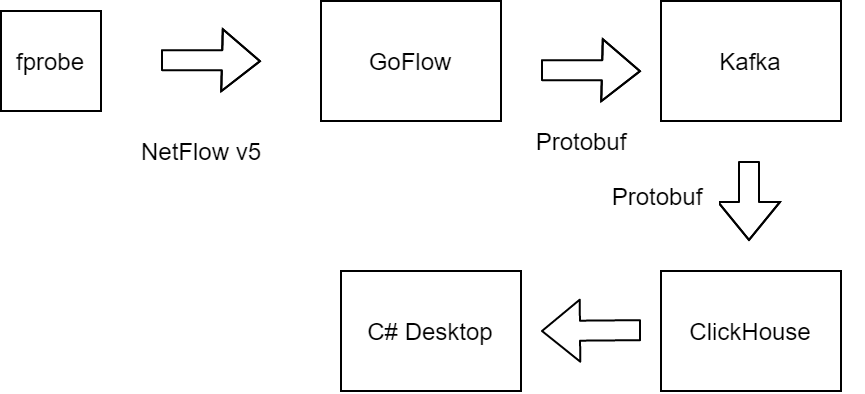
\includegraphics[scale=0.55]{concp.png}
	\caption{Схема потоков данных системы.}
	\label{DataFlowEnd}
\end{figure}

\subsection{Создание базы данных}

Специфика Clickhouse наложила некоторые ограничения. Clickhouse не поддерживает PrimaryKey и ForeignKey, не поддерживает уникальность значений в таблице, отсутствует поддержка транзакций и другие особенности\cite{clickhouse}. В связи с этим нельзя сказать, что одна таблица ссылается на другую и нельзя построить диаграмму БД. На рисунке \ref{img:DB} представлены сущности БД. \\
\begin{figure}[H]
	\centering
	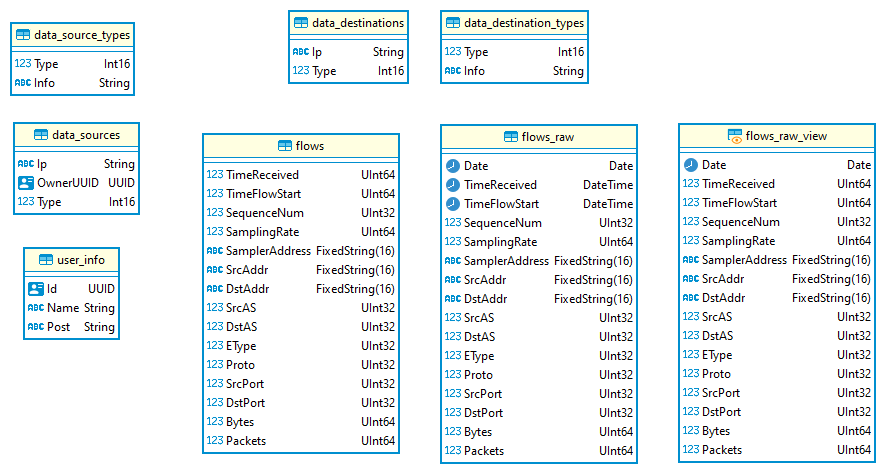
\includegraphics[scale=0.55]{images/bd.png}
	\caption{Диаграмма БД.}
	\label{img:DB}
\end{figure}

\subsubsection{Описание полей базы данных}
В таблице flows представлена часть структуры Netflow пакета, значения полей которого определяются стандартом Netflow. Из полученного пакета будут выбраны следующие поля:
\begin{itemize}
	\item TimeReceived - Время получения пакета
	\item TimeFlowStart - Время начала потока
	\item SequenceNum - Время пакета в текущей записываемой последовательности
	\item SamplingRate - Пакеты для семплирования
	\item SamplerAddres - Адресс семплера потока
	\item SrcAddr - Адресс источника пакета
	\item DstAddr - Адрес назначения пакета
	\item SrcAS - BGP автономной системы
	\item DstAS - BGP автономной системы	
	\item EType - Протокол третьего уровня
	\item Proto - Протокол четвертого уровня
	\item SrcPort - Порт источника
	\item DstPort - Порт назначения
	\item Bytes - Размер потока в байтах
	\item Packets - Количество агрегированных пакетов
\end{itemize}
\indent Материализованное представление flow\_raw\_view и таблица flows\_raw дублируют эти поля, добавляя поле Date - Дату получения пакета. \\
\indent Остальные таблицы хранят информацию для категорирования входящих пакетов. Таблица data\_sources - хранит адрес источника пакета, тип источника и UUID владельца источника. Таблица data\_sources\_type - хранит типы источников. Таблица data\_destinations - хранит адрес назначения пакета и его тип. Таблица data\_destinations\_type - хранит типы назначений.
\subsubsection{Типы таблиц}
В базе данных используется три типа таблиц.
\subsubsubsection{Движок Kafka}
В ClickHouse Существует понятие движка(engine), который определяет:
\begin{itemize}
\item как и где хранятся данные, куда их писать и откуда читать;
\item какие запросы поддерживаются и каким образом;
\item конкурентный доступ к данным;
\item использование индексов, если есть;
\item возможно ли многопоточное выполнение запроса;
\item параметры репликации данных.
\end{itemize}

Движок Kafka определяет, что данные берутся из Kafka и записываются в таблицу. Рассмотри создание таблицы на листинге \ref{flowsLst}.
\begin{lstlisting}[label={flowsLst}, language=SQL]
CREATE TABLE IF NOT EXISTS flows
(
    TimeReceived UInt64,
    TimeFlowStart UInt64,
    SequenceNum UInt32,
    SamplingRate UInt64,
    SamplerAddress FixedString(16),
    SrcAddr FixedString(16),
    DstAddr FixedString(16),
    SrcAS UInt32,
    DstAS UInt32,
    EType UInt32,
    Proto UInt32,
    SrcPort UInt32,
    DstPort UInt32,
    Bytes UInt64,
    Packets UInt64
)
ENGINE = Kafka
SETTINGS kafka_broker_list = '192.168.1.53:9092',
 kafka_topic_list = 'flows',
 kafka_group_name = 'clickhouse',
 kafka_format = 'Protobuf',
 kafka_schema = './flow.proto:FlowMessage';
\end{lstlisting}
В строках 2-17 определяется структура таблицы, в строке 18 указывается, что используется движок Kafka. В строках 19-23 определяются следующие настройки:
\begin{itemize}
\item kafka\_broker\_list - список адресов брокеров Kafka
\item kafka\_topic\_list - название топика Kafka;
\item kafka\_group\_name - название группы при подключении;
\item kafka\_format - формат получаемых данных;
\item kafka\_schema - схема получаемых данных.
\end{itemize}

\subsubsubsection{Материализованное представление}
Таблица flows\_raw\_view является материализованным представлением.
Рассмотрим создание таблицы на листинге \ref{flowsVLst}.
\begin{lstlisting}[label={flowsVLst}, language=SQL]
CREATE MATERIALIZED VIEW IF NOT EXISTS default.flows_raw_view TO default.flows_raw
(
    `Date` Date,
    `TimeReceived` UInt64,
    `TimeFlowStart` UInt64,
    `SequenceNum` UInt32,
    `SamplingRate` UInt64,
    `SamplerAddress` FixedString(16),
    `SrcAddr` FixedString(16),
    `DstAddr` FixedString(16),
    `SrcAS` UInt32,
    `DstAS` UInt32,
    `EType` UInt32,
    `Proto` UInt32,
    `SrcPort` UInt32,
    `DstPort` UInt32,
    `Bytes` UInt64,
    `Packets` UInt64
) AS
SELECT
    toDate(TimeReceived) AS Date, *
FROM default.flows;
\end{lstlisting}
В строке 1 указывается, что создается материализованное представление, результат которого будет вставлен в таблицу flows\_raw. MATERIALIZED - Материализованное выражение, всегда вычисляется.\\
Строки 2-18 описывают строение. Далее идет описание SELECT из default.flows.
\subsubsubsection{Обычная таблица}
Таблица flows\_raw создается как обычная таблица. Рассмотрим создание таблицы на листинге \ref{flowsRawLst}.
\begin{lstlisting}[label={flowsRawLst}, language=SQL]
CREATE TABLE IF NOT EXISTS flows_raw
(
    Date Date,
    TimeReceived DateTime,
    TimeFlowStart DateTime,
    SequenceNum UInt32,
    SamplingRate UInt64,
    SamplerAddress FixedString(16),
    SrcAddr FixedString(16),
    DstAddr FixedString(16),
    SrcAS UInt32,
    DstAS UInt32,
    EType UInt32,
    Proto UInt32,
    SrcPort UInt32,
    DstPort UInt32,
    Bytes UInt64,
    Packets UInt64
)
ENGINE = MergeTree
PARTITION BY Date
ORDER BY TimeReceived;
\end{lstlisting}
В данном случае используется движок MergeTree. Движок MergeTree, а также другие движки этого семейства (*MergeTree) — это наиболее функциональные движки таблиц ClickHouse. \\
Основная идея, заложенная в основу движков семейства MergeTree следующая. Когда у вас есть огромное количество данных, которые должны быть вставлены в таблицу, вы должны быстро записать их по частям, а затем объединить части по некоторым правилам в фоновом режиме. Этот метод намного эффективнее, чем постоянная перезапись данных в хранилище при вставке\cite{clickhouse-mergetree}. \\
\indent Строка PARTITION BY Date указывает, что создается партицирование по ключу Date. ClickHouse поддерживает операции над партициями, которые намного эффективнее обычных. Так же, если задан ключ партицирования в запросе, ClickHouse сразу выберет нужную партицию, что также увеличивет эффективность выполнения запросов. \\
\indent Создание остальных таблиц приведено в приложении A.


В данном случае таблица flows напрямую берет данные из Kafka, но не хранит в себе данные предыдущего запроса к Kafka, а только последнего. Таблица же flows\_raw, дублируя flows, не удаляет старые данные при получении новых. Синхронизировать запись в flows\_raw при добавлении во flows помогает flows\_raw\_view - материализованное представление, ещё одна особенность Clickhouse. В Clickhouse отсутствуют триггеры и функции, определяемые пользователем, но вместо этого существуют материализованные представления, которые работают схожим образом с триггером добавления.
\subsection{Разработка компонентов}
При разработке приложения были встречены трудности, так же обусловленные выбором Clickhouse.
\subsubsection{Компонент доступа к данным}
В C\# есть фрэймворк EntityFramework и его модули, предоставляющие ORM для многих популярных баз данных, тем самым существенно упрощая процесс разработки. Но для Clickhouse нет готовой ORM, поэтому компонент доступа данным использует query билдеры.
На рисунке \ref{img:AccessToDB} представлена UML-диаграмма компонента доступа к данным.
\begin{figure}[H]
	\centering
	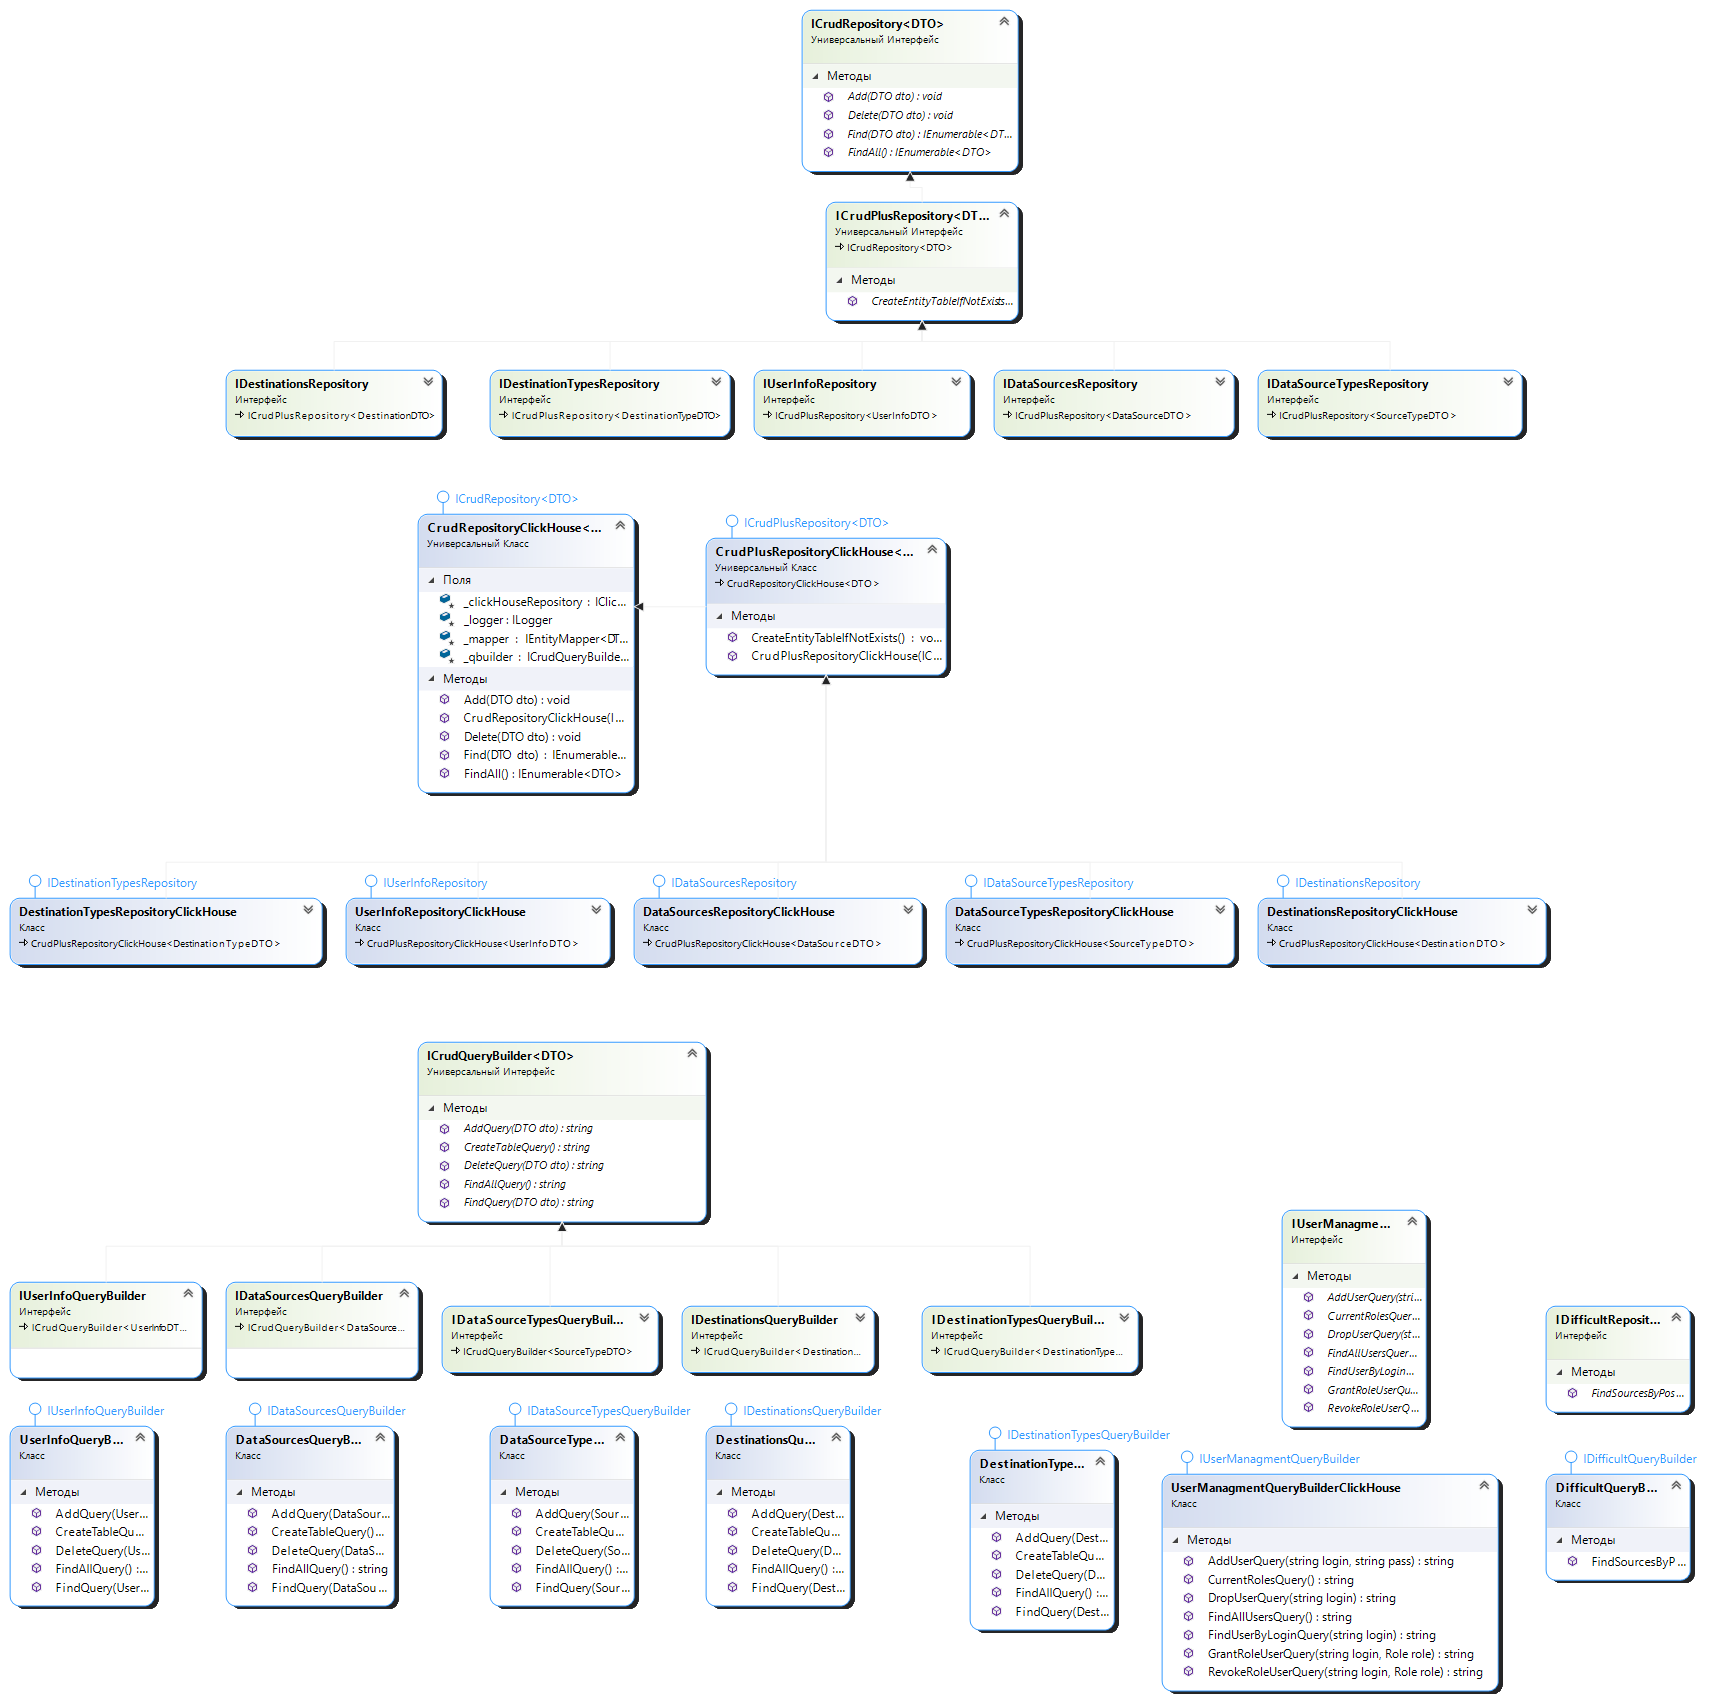
\includegraphics[scale=0.35]{AccessToDB.png}
	\caption{Компонент доступа к данным.}
	\label{img:AccessToDB}
\end{figure}
\subsubsection{Компонент бизнес-логики}
На рисунке \ref{img:Controllers} представлена UML-диаграмма компонента бизнес-логики.
\begin{figure}[H]
	\centering
	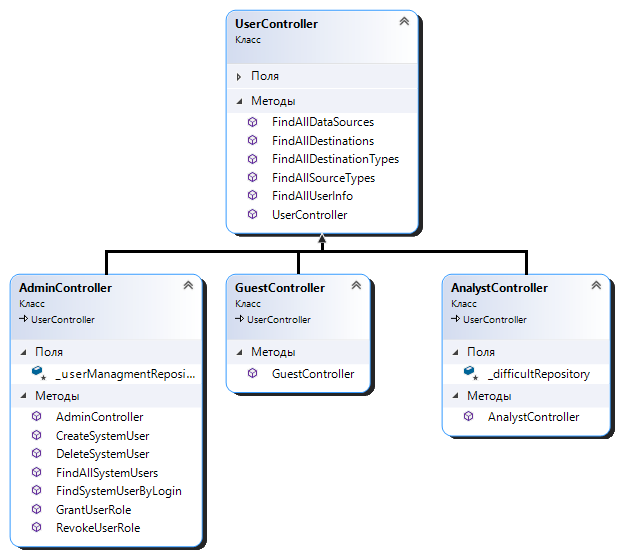
\includegraphics[scale=1]{Controllers.png}
	\caption{Компонент бизнес-логики.}
	\label{img:Controllers}
\end{figure}
\subsection{Интерфейс приложения}
На рисунках ниже показан пользовательский интерфейс.
\begin{figure}[H]
	\centering
	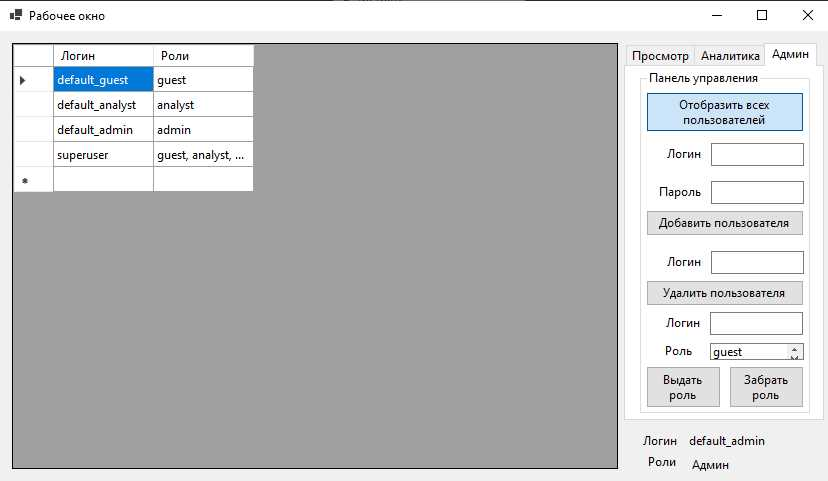
\includegraphics[scale=0.75]{admin.jpg}
	\caption{Вкладка админа.}
	\label{img:analytic}
\end{figure}
\indent На этой вкладке можо получить доступ к функциям админа, добавлению и удалению пользователей, выдачу и отзыв ролей.
\begin{figure}[H]
	\centering
	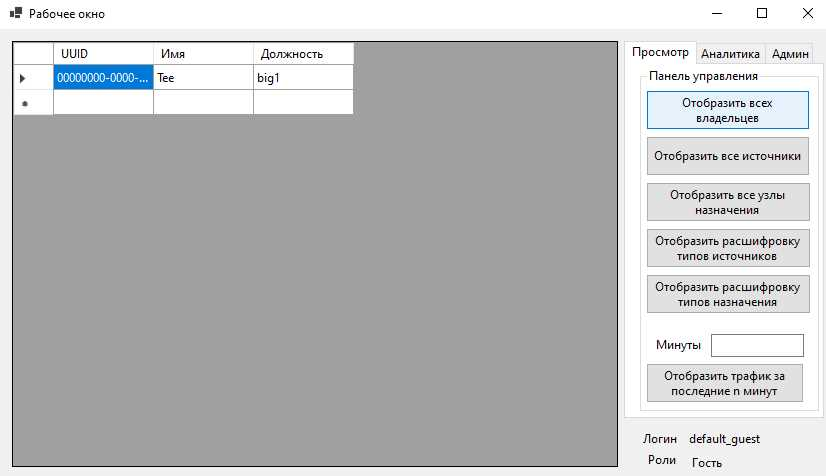
\includegraphics[scale=0.75]{guest.jpg}
	\caption{Общедоступная вкладка.}
	\label{img:manager}
\end{figure}
\indent На этой вкладке можо получить доступ к функциям гостя. Каждый пользователь может это сделать. К функциям гостя относят только базовые функции для просмотра данных.
\subsection{Docker}
При развертовании системы был использован докер, что позволит разворачивать и настраивать систему не зависимо от машины, упрастит масштабирование.
\subsection{Вывод}
В данном разделе были выбраны средства реализации поставленной задачи, создана база данных, разработано приложение.
\newpage
\section*{Заключение}
\addcontentsline{toc}{section}{Заключение}
В процессе выполнения курсовой работы задание было выполнено следующее:
\begin{itemize}
\item проведен анализ предметной области;
\item были выбраны подходящие инструменты для решения задачи;
\item реализован программный комплекс;

\end{itemize}

\indent Цель курсовой работы достигнута, все задачи выполнены. \\

В процессе разработки была заложена возможность масштабирования системы. В качестве дальнейшего развития можно предложить:
\begin{itemize}
\item введение системы в эксплуатацию;
\item добавление возможности управлять сенсором через приложение;
\item доработка UI приложения и логики добавления новых запросов.
\end{itemize}

\clearpage
%СПИСОК ЛИТЕРАТУРЫ
\begin{thebibliography}{9}
	\addcontentsline{toc}{section}{Литература}
	\bibitem{netflow} Introduction to Cisco IOS NetFlow [Электронный ресурс] URL: https://www.cisco.com/c/en/us/products/collateral/ios-nx-os-software/ios-netflow/prod\_white\_paper0900aecd80406232.html (дата обращения: 09.06.2021).
	\bibitem{wireshark} Wireshark [Электронный ресурс] URL: https://www.wireshark.org/ (дата обращения: 09.06.2021).
	\bibitem{tcpdump} Man page of tcpdump [Электронный ресурс] URL: https://www.tcpdump.org/manpages/tcpdump.1.html (дата обращения: 09.06.2021).
	\bibitem{elastic} Elasticksearch as NoSQL [Электронный ресурс] URL:  https://www.elastic.co/blog/found-elasticsearch-as-nosql (дата обращения: 09.06.2021).
	\bibitem{clickhouse} ClickHouse : Введение [Электронный ресурс] URL: https://clickhouse.tech/docs/ru/introduction/distinctive-features/ (дата обращения: 09.06.2021).
	\bibitem{clickhouse-kafka} ClickHouse : Kafka [Электронный ресурс] URL: https://clickhouse.tech/docs/en/engines/table-engines/integrations/kafka/ (дата обращения: 09.06.2021).
	\bibitem{clickhouse-elastic} ClickHouse vs Elasticsearch [Электронный ресурс] URL: https://altinity.com/faqs/clickhouse-and-elasticsearch-faqs (дата обращения: 09.06.2021).
	\bibitem{kafka-redis} Kafka vs Redis [Электронный ресурс] URL: https://www.upsolver.com/blog/kafka-versus-rabbitmq-architecture-performance-use-case (дата обращения: 10.06.2021).
	\bibitem{sharp} Документация по C\# [Электронный ресурс] URL: https://docs.microsoft.com/ru-ru/dotnet/csharp/ (дата обращения: 09.06.2021).
	\bibitem{vs} Документация по семейству продуктов Visual Studio [Электронный ресурс] URL: https://docs.microsoft.com/ru-ru/visualstudio/?view=vs-2019 (дата обращения: 09.06.2021).
	\bibitem{clickhouse-mergetree} ClickHouse : MergeTree [Электронный ресурс] URL:https://clickhouse.tech/docs/ru/engines/table-engines/mergetree-family/mergetree (дата обращения: 10.06.2021).
\end{thebibliography}

 \clearpage
 {\centering\textbf{Приложение А.} \par}
 {\centering Создание таблиц базы данных. \par}
 \addcontentsline{toc}{section}{Приложение А. Создание таблиц базы данных.}
\begin{lstlisting}[label={lst:appA}, language=SQL]   
CREATE TABLE IF NOT EXISTS data_sources (
                        Ip String,
                        OwnerUUID UUID,
                        Type Int16
                        )
                        ENGINE=MergeTree()
                        ORDER BY (Ip);
                        
CREATE TABLE IF NOT EXISTS data_source_types (
                        Type Int16,
                        Info String
                        )
                        ENGINE=MergeTree()
                        ORDER BY (Type);
                       
   CREATE TABLE IF NOT EXISTS data_destinations (
                        Ip String,
                        Type Int16
                        )
                        ENGINE=MergeTree()
                        ORDER BY (Ip);
                       
   CREATE TABLE IF NOT EXISTS data_destination_types (
                        Type Int16,
                        Info String
                        )
                        ENGINE=MergeTree()
                        ORDER BY (Type);
                       
   CREATE TABLE IF NOT EXISTS user_info (
                        Id UUID,
                        Name String,
                        Post String
                        )
                        ENGINE=MergeTree()
                        ORDER BY (Id);
\end{lstlisting}
 \newpage
\addcontentsline{toc}{section}{Приложение Б. Презентация.}
 {\centering\textbf{Приложение Б. Презентация} \par}
\begin{figure}[H]
	\centering
	
\includegraphics[scale=0.35]{pr1.jpg}
\end{figure}
\begin{figure}[H]
	\centering
	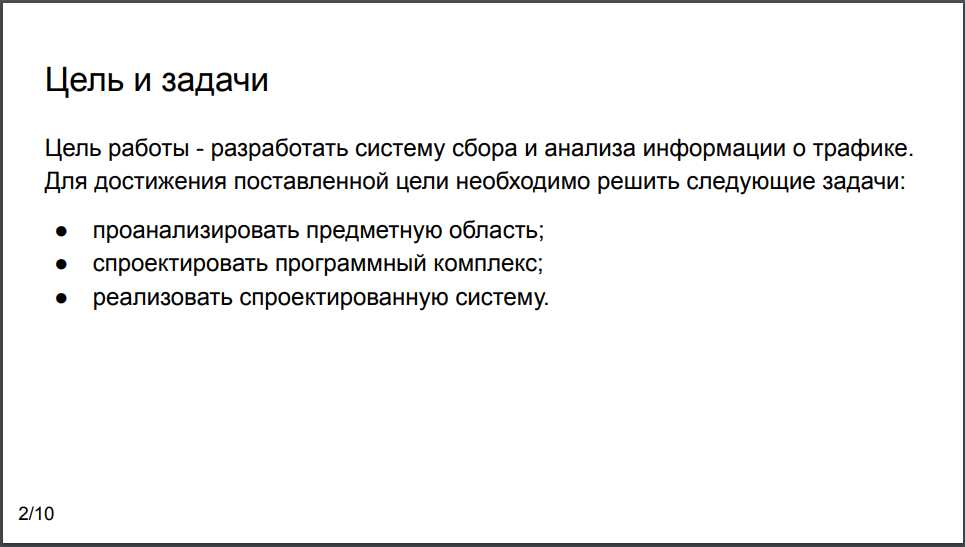
\includegraphics[scale=0.35]{pr2.jpg}
\end{figure}
\begin{figure}[H]
	\centering
	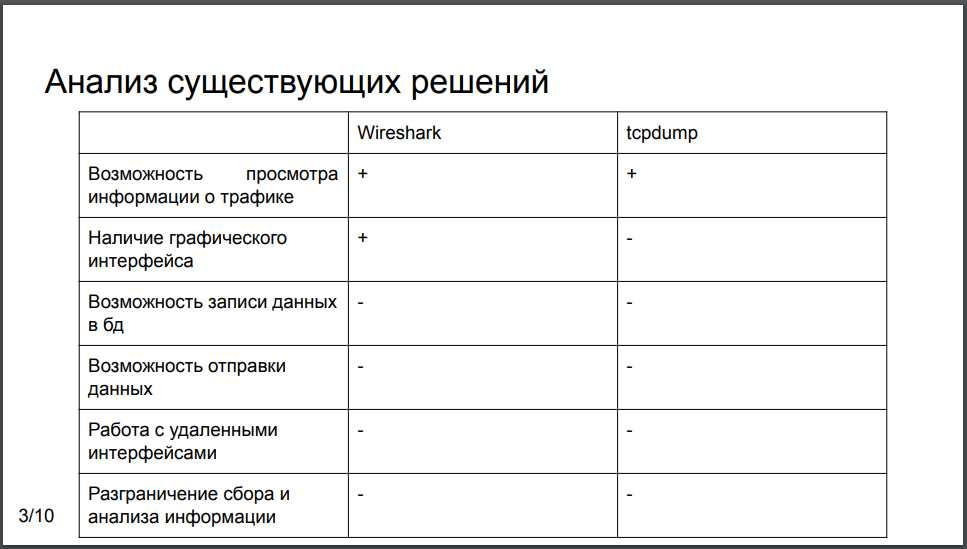
\includegraphics[scale=0.35]{pr3.jpg}
\end{figure}
\begin{figure}[H]
	\centering
	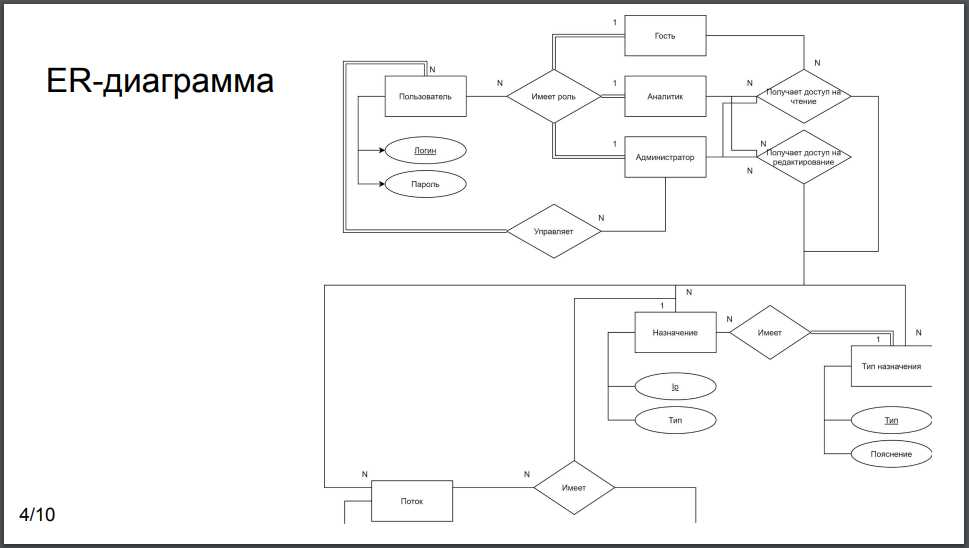
\includegraphics[scale=0.35]{pr4.jpg}
\end{figure}
\begin{figure}[H]
	\centering
	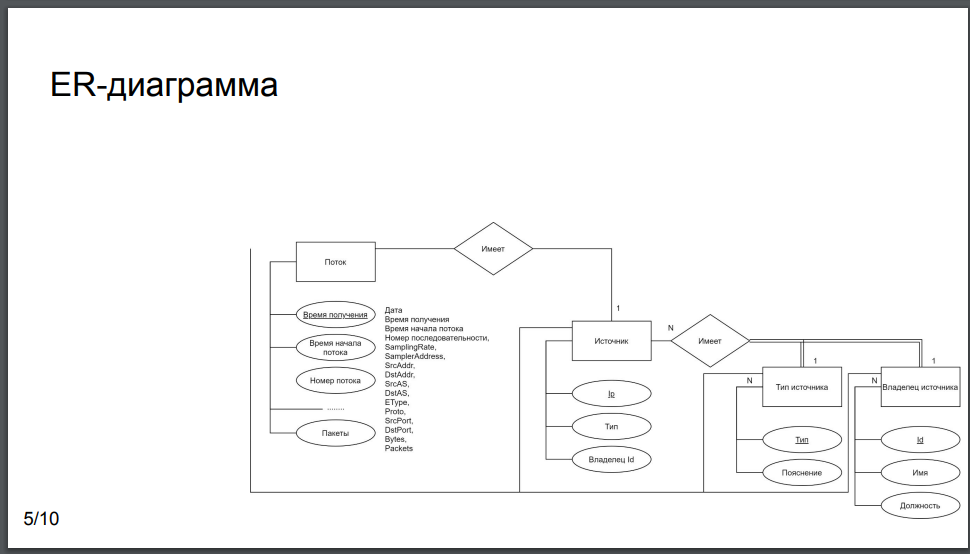
\includegraphics[scale=0.35]{pr5.jpg}
\end{figure}
\begin{figure}[H]
	\centering
	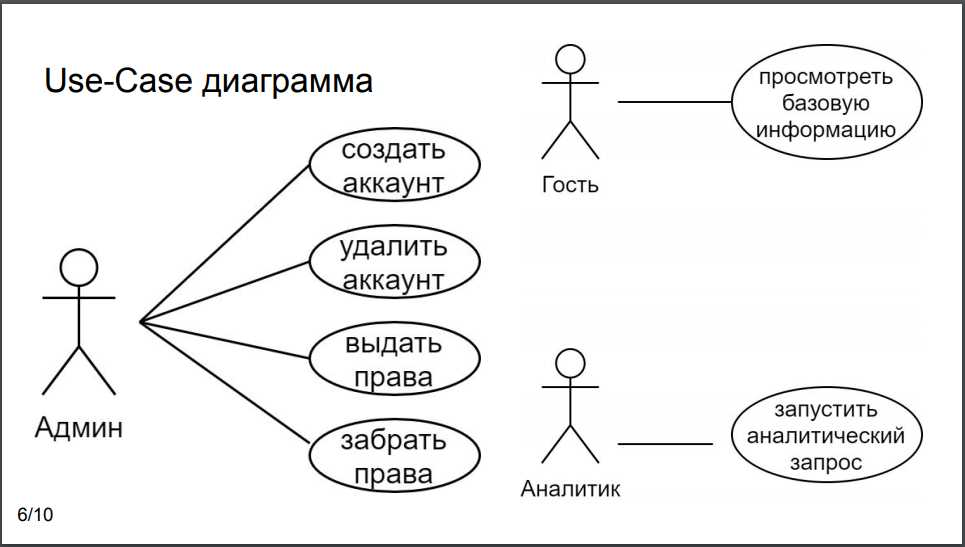
\includegraphics[scale=0.35]{pr6.jpg}
\end{figure}
\begin{figure}[H]
	\centering
	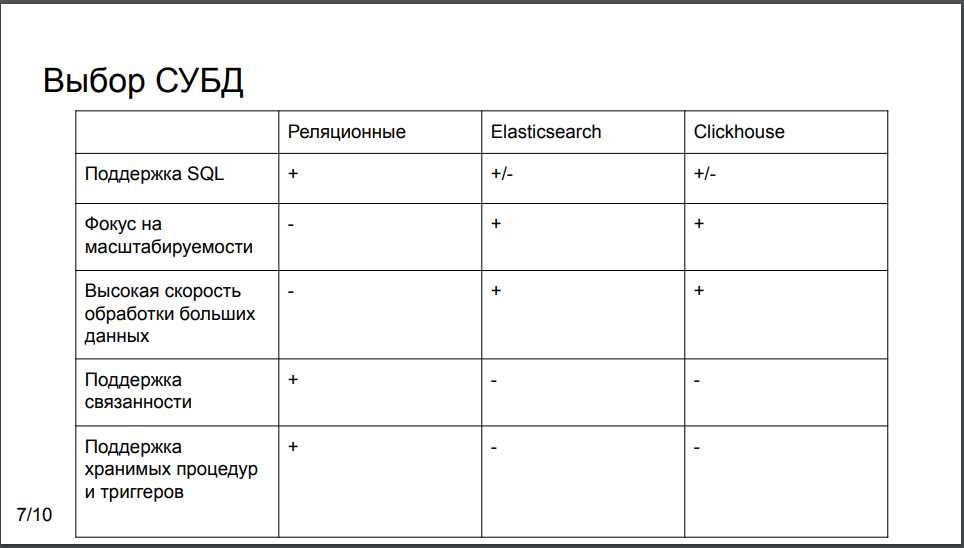
\includegraphics[scale=0.35]{pr7.jpg}
\end{figure}
\begin{figure}[H]
	\centering
	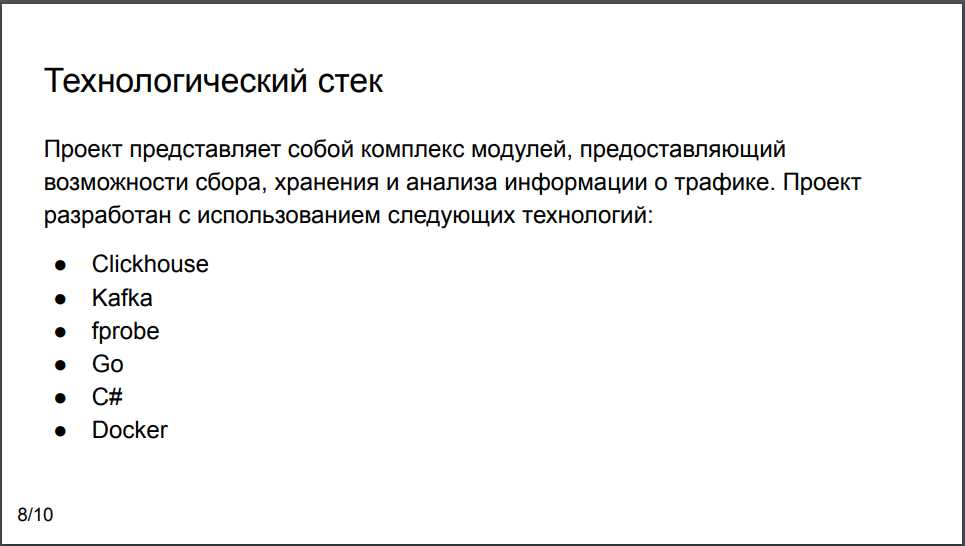
\includegraphics[scale=0.35]{pr8.jpg}
\end{figure}
\begin{figure}[H]
	\centering
	
\includegraphics[scale=0.35]{pr9.jpg}
\end{figure}
\begin{figure}[H]
	\centering
	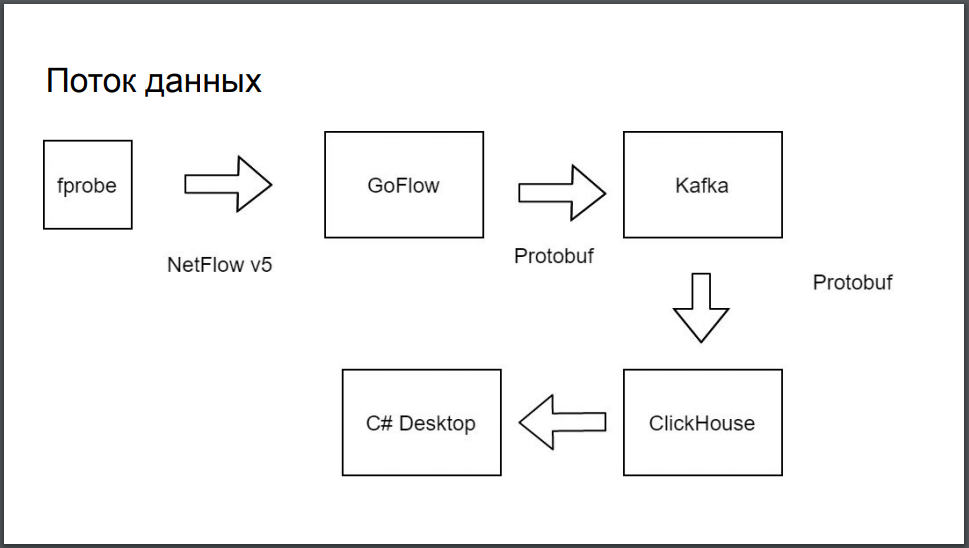
\includegraphics[scale=0.35]{prf.png}
\end{figure}
\begin{figure}[H]
	\centering
	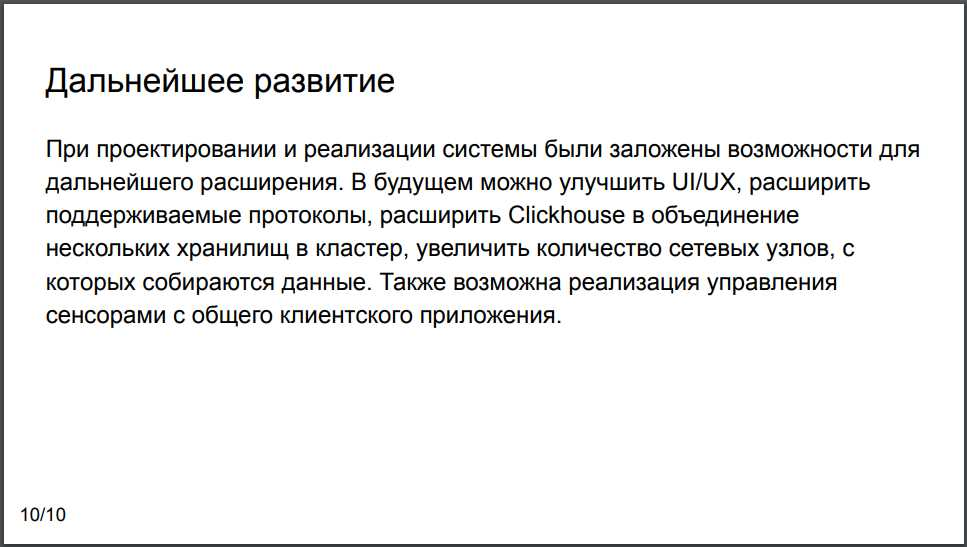
\includegraphics[scale=0.35]{pr10.jpg}
\end{figure}
\begin{figure}[H]
	\centering
	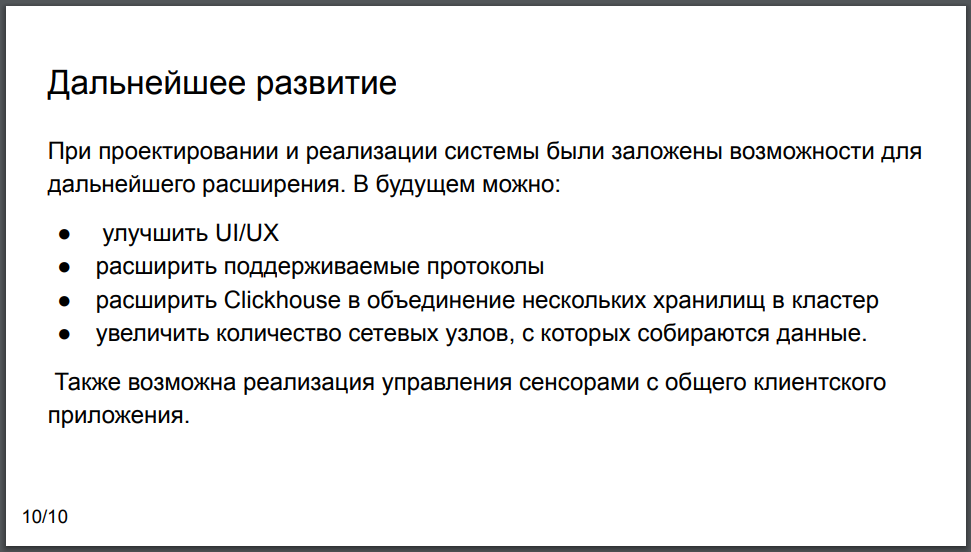
\includegraphics[scale=0.35]{pr11.png}
\end{figure}
\end{document}